% !TEX root = ../main.tex

% Exercises section

\section{Exercises}

\subsection{Exercise 1: Threshold Function}
Consider we have a class of threshold functions $\mathcal{H} = { 0.1 , 0.2 ,..., 0.9 }$, and let $x \in \mathbb R$ lies in the interval [0, 1]. For example, one of the members of  $\mathcal{H}$  is the function:
\[
  h_{\theta = 0.1}(x) =
  \begin{cases}
                                   1 & \text{if $x > theta$ }\\
                                   0 & \text{if $x < theta$ } 
  \end{cases}
\]
\begin{enumerate}
    \item what training set size we need for PAC learning for $\varepsilon = 0.01$ and %\delta = 0.05%?
    \item what if we increase $\varepsilon$
\end{enumerate}

\subsubsection{Solution for Exercise 1}
\begin{enumerate}
    \item From the section ``Learning any function", we have $m \geq \frac{2}{\varepsilon^{2}}(\ln2|\mathcal{H}|+\ln \frac{1}{delta})$. Plugging in each elements, we have $m \geq \dfrac{2}{0.01^{2}}()\ln 18 + ln\frac{1}{0.05} \approx 117722$.
    \item Repeating the steps below, $m \geq \dfrac{2}{0.1^{2}}()\ln 18 + ln\frac{1}{0.05} \approx 117723$. We can observed that even though the $\varepsilon$ become $10$ times large, there isn't an obvious change in sufficient sample size.
\end{enumerate}


\subsection{Exercise 2:  Understanding the Concept of PAC Learning}
\begin{enumerate}
    \item Please judge whether the statements below is true or false.
\begin{enumerate}
    \item  In a PAC learning model, the learner makes no assumptions about the class from which the target concept is drawn. 
    \item The number of training examples required for successful learning is strongly influenced by the complexity of the hypothesis space considered by the learner.
    \item In PAC learning, the learner outputs the hypothesis from $\mathcal{H}$ that has the lowest error over the training data.
\end{enumerate}
    \item Suppose $\mathcal{H}$ is a finite hypotheses class and $\mathcal{S}$ is a set of training data. We would like our algorithm to output the most probable hypothesis $h \in \mathcal{H}$, given the data  $\mathcal{S}$. Under what conditions does the following hold?
    \begin{equation*}
        \operatorname{argmax}_{h \in \mathcal{H}}P(h|\mathcal{D}) = \operatorname{argmax}_{h \in \mathcal{H}}P(\mathcal{D}|h)
    \end{equation*}
\end{enumerate}

\subsubsection{Solution for Exercise 2}
\begin{enumerate}
    \item True/False?
    \begin{enumerate}
    \item False
    \item True
    \item False
\end{enumerate}
    \item Conditions: $P(\mathcal{D})$ can be dropped because it does not depend on h
$P(h)$ can be treated as a constant if all the hypotheses in the hypothesis space are equally likely.

\end{enumerate}






\subsection{Exercise 3:  PAC Learning}
After drop the realizability assumption that there is a hypothesis in H with zero true error, and move to agnostic PAC-learning. Let $\mathcal{H}$ be finite class. If we require
$$
\mathbb{P}_{D \sim \mathbb{P}(X, Y)^{m}}\left[\operatorname{err}_{\mathcal{D}}\left(h_{D}\right)>\min _{h \in \mathcal{H}}\left\{\operatorname{err}_{\mathcal{D}}(h)\right\}+\epsilon\right] \leq \delta
$$
where $h_{D}$ is any hypothesis output by an ERM learner, then it suffices to obtain a sample that is $\frac{\epsvarepsilonilon}{2}$ representative with probability at least $1-\delta .$ That is, we need
$$
\mathbb{P}_{D \sim \mathbb{P}(X, Y)^{m}}\left[\exists h \in \mathcal{H}:\left|\operatorname{err}_{\mathcal{D}}(h)-\operatorname{err}_{D}(h)\right|>\frac{\varepsilon}{2}\right] \leq \delta
$$
By the union bound and Hoeffding's inequality we have that
$$
\mathbb{P}_{D \sim \mathbb{P}(X, Y)^{m}}\left[\exists h \in \mathcal{H}:\left|\operatorname{err}_{\mathcal{D}}(h)-\operatorname{err}_{D}(h)\right|>\frac{\varepsilon}{2}\right] \leq 2|\mathcal{H}| e^{-\frac{1}{2} \varepsilon^{2} m}
$$
Hence, we need $\delta \geq 2|\mathcal{H}| e^{-\frac{1}{2} \varepsilon^{2} m}$. 

\begin{enumerate}
    \item Derive a formula for the sufficient sample size to meet given $(\varepsilon,\delta)$ requirements. Compare this to the sample size that with the realizability assumption and explain the difference.
    \item A data set D is called $\varepsilon$-representative w.r.t. domain $Z$, hypothesis class $\mathcal{H}$,  and distribution  $\mathcal{D}$ if 
    \begin{equation*}
        \forall h \in \mathcal{H}:\left|\operatorname{err}_{D}(h)-\operatorname{err}_{\mathcal{D}}(h)\right| \leq \epsilon
    \end{equation*}\cite{Siebes}
     Show that if the sample is $2\varepsilon$ representative with respect to $\mathcal{H}$, then $\operatorname{err}(h_{\mathcal{D}}) \leq \operatorname{min}_{h \in \mathcal{H}}{\operatorname{err}_{\mathcal{D}}(h)} + \varepsilon$, for any ERM hypothesis is $h_{\mathcal{D}}$.

\end{enumerate}

\subsubsection{Solution for Exercise 3}
\begin{enumerate}
    \item Starting from $\delta \geq 2|\mathcal{H}|e^{-0.5\varepsilon^{2}m}$, we solve for $m$ and get:
\begin{equation*}
    m \geq \frac{2}{\varepsilon^{2}}\left(\ln 2|\mathcal{H}|+\ln \frac{1}{\delta}\right)
\end{equation*}
For the one with realizability assumption, 
\begin{equation*}
    m \geq \frac{1}{\varepsilon}\left(\ln 1|\mathcal{H}|+\ln \frac{1}{\delta}\right)
\end{equation*}
The most important difference is that in the agnostic case (without the realizability assumption) we have the factor $\frac{2}{\varepsilon^{2}}$
instead of 1ε in the realizable case. Since $\varepsilon \in (0,1)$, and typically closer to 0, we have that $\varepsilon^{2}$ is smaller than $\varepsilon$, and hence $\frac{1}{\varepsilon^{2}}$ is bigger than $\frac{1}{\varepsilon}$ . The rule is that we need more data in the agnostic case.\\
    \item The idea of this question can be acquired from this image:
    \begin{figure}[h]
        \centering
        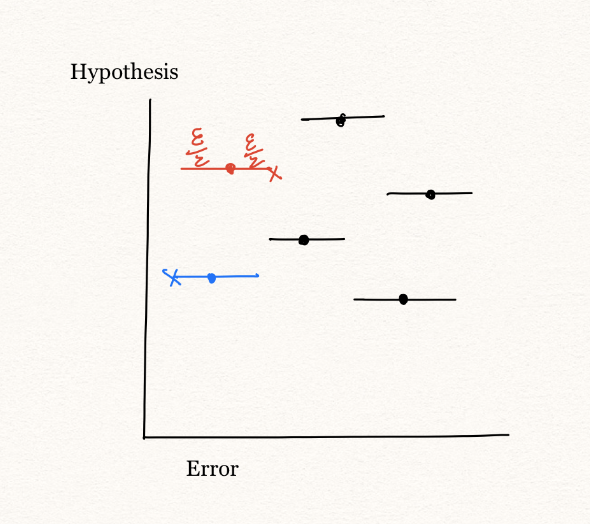
\includegraphics[scale = 0.4]{misc/ex_2.png}
        \caption{Agnostic PAC-learning}
        \label{fig:my_label}
    \end{figure}
The dots are the training error of different hypotheses. Since the sample is $2-\varepsilon$ representative, we know that the true error is within $2-\varepsilon$ of the training error. Our ERM-algorithm will return a hypothesis with minimum training error. In the picture, both the red and the blue hypothesis achieve the minimum training error, so an ERM algorithm choose either one of them. If our ERM algorithm returns the red one. Worst thing that can happen is that its true error (the red cross) is $2-\varepsilon$ higher than its training error, but for the blue hypothesis, the true error (the blue cross) is $2-\varepsilon$ smaller than its training error. However, the true error of the selected hypothesis is still within $\varepsilon$ of the best true error. Expressing in inequalities: for any $h \in \mathcal{H}$:
\begin{equation*}
    \begin{split}
     \operatorname{err}_{D}(h_{D}) &\leq \operatorname{err}_{D}(h_{D})+\frac{\varepsilon}{2}\\
     & \leq \operatorname{err}_{D}(h)+\frac{\varepsilon}{2}\\
     & \leq \operatorname{err}_{D}(h)+\frac{\varepsilon}{2}+\frac{\varepsilon}{2}\\
     & = \operatorname{err}_{D}(h)+\varepsilon
    \end{split}
\end{equation*}
Hence, on an $\frac{\varepsilon}{2}$-representative sample $D$, the $\text{ERM}_{\mathcal{H}}$-rule yields an optimal result. 

\end{enumerate}

